\subsection*{Marco conceptual del proyecto}

\subsubsection*{Mezcla de audio}

La mezcla de audio es una de las etapas más determinantes dentro del proceso de producción musical. En términos técnicos, consiste en combinar múltiples pistas individuales, cada una con su propia dinámica, timbre y contenido espectral, para obtener una versión final equilibrada y coherente de una obra sonora. Como describen De Man, Reiss y Stables en [4], las pistas grabadas casi siempre requieren un procesamiento considerable antes de estar listas para su distribución, que incluye balance de niveles, paneo, ecualización (EQ), compresión de rango dinámico y reverberación artificial.

Lo que hace a la mezcla un proceso complejo es que no existe una única solución correcta. Múltiples ingenieros pueden abordar el mismo material y llegar a resultados igualmente válidos dependiendo de sus criterios estéticos, el género musical y la intención artística del proyecto. Esta naturaleza abierta del proceso fue descrita por Moliner et al. en [3], quien señaló que la mezcla es una tarea caracterizada por la subjetividad, donde existen múltiples soluciones válidas para un mismo conjunto de pistas. Por esta razón, los sistemas automáticos que tratan la mezcla como un problema de estándares por géneros, es decir, que intentan predecir una única mezcla "correcta" en base a un estándar y no a la necesidad de la grabación, tienden a producir resultados planos y poco expresivos.

Desde la perspectiva práctica, el proceso de mezcla abarca decisiones en distintos niveles: el control de gain staging y balance de faders, la gestión espectral mediante EQ, el control dinámico a través de compresores y limitadores, la construcción del espacio sonoro con reverberación y delay, y el uso de efectos creativos como saturación o modulación. Todas estas decisiones son interdependientes; modificar un parámetro en una pista puede afectar la percepción del conjunto. Esta interdependencia fue descrita con precisión por Martínez Ramírez, Stoller y Moffat en [2], quienes afirman que todos los aspectos y parámetros de una mezcla están inherentemente entrelazados e interrelacionados.

\subsubsection*{Mezcla vocal}

Dentro del proceso de mezcla general, la mezcla vocal ocupa un lugar especialmente relevante. La voz humana es el elemento central en la mayoría de los géneros musicales populares, y su tratamiento busca lograr claridad, inteligibilidad y presencia dentro del conjunto sonoro de la canción sin que pierda su carácter ni se desvincule del arreglo instrumental que la acompaña.

El procesamiento vocal típicamente se organiza en cadenas de efectos secuenciales en las que el orden y la configuración de cada herramienta afectan directamente el resultado final. Una cadena de mezcla vocal puede incluir filtros de paso alto para eliminar frecuencias indeseadas en los graves, ecualizadores paramétricos para moldear el timbre, compresores para controlar la dinámica y homogeneizar la presencia, de-essers para reducir sibilancias excesivas, saturadores para añadir armónicos que den calidez, y efectos de tiempo como reverberación y delay para posicionar la voz en un espacio sonoro determinado. La elección de estos procesos y de sus parámetros no responde a una fórmula fija: depende de las características acústicas de la voz grabada, del estilo musical y de las decisiones creativas del ingeniero.

\begin{figure}[h!]
\centering
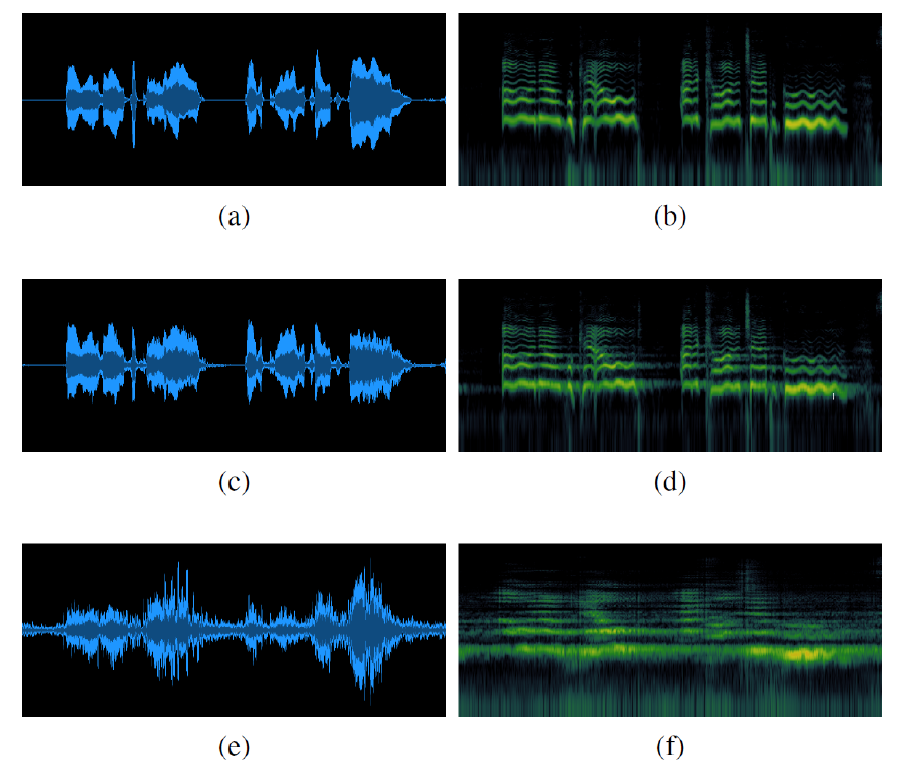
\includegraphics[width=0.8\textwidth]{images/fig1.png} 
\caption{Comparación de forma de onda y espectrograma entre grabación vocal cruda (entrada) y stem procesado (salida objetivo) en el sistema DAE. Fuente: Martínez Ramírez y Reiss [5].}
\label{fig:fig1}
\end{figure}

Esta diversidad de configuraciones posibles genera una brecha de incertidumbre importante, especialmente para productores con menor experiencia. Como señala el trabajo de Vanka et al. en [1], muchos productores en contextos de home studio enfrentan la mezcla sin formación profesional, lo que los lleva a trabajar mediante ensayo y error, lo cual prolonga los tiempos de producción y genera resultados inconsistentes.

\subsubsection*{Inteligencia artificial aplicada al audio}

La inteligencia artificial hace referencia al desarrollo de sistemas computacionales capaces de analizar datos, identificar patrones y tomar decisiones sin ser programados de manera explícita para cada caso. En el campo del audio y la producción musical, estas tecnologías han ganado terreno de manera constante en los últimos años, impulsadas por el crecimiento del aprendizaje profundo y la disponibilidad de grandes volúmenes de datos de audio.

Dentro de las técnicas más utilizadas se encuentran las redes neuronales profundas (DNN), que han demostrado ser capaces de aprender transformaciones complejas directamente desde señales de audio. Martínez Ramírez y Reiss, en [5], propusieron desde 2017 una investigación centrada en el uso de autoencoders profundos para aprender cadenas de efectos de audio como transformaciones basadas en contenido, siguiendo arquitecturas de extremo a extremo donde el audio crudo es tanto la entrada como la salida del sistema.

Un aspecto fundamental para el desarrollo de sistemas inteligentes de asistencia en mezcla vocal es la capacidad de analizar y cuantificar las características acústicas de la voz de manera objetiva. Chen en [6], investigó el uso de tecnologías de procesamiento digital de señales y machine learning para el entrenamiento vocal asistido por computador, demostrando que parámetros como la frecuencia fundamental, la relación armónico-ruido (HNR) y los coeficientes mel-frequency cepstral (MFCC) permiten evaluar y retroalimentar el desempeño vocal con mayor precisión que los métodos tradicionales. En un experimento con 60 participantes durante 12 semanas, el grupo entrenado con asistencia computacional mostró mejoras en precisión de pitch casi el doble de las obtenidas con métodos convencionales, lo que evidencia que la cuantificación de parámetros acústicos vocales es no solo viable sino significativamente más efectiva para orientar procesos de ajuste técnico [6]. Aunque el contexto de ese trabajo es pedagógico, los parámetros acústicos identificados son igualmente relevantes para un sistema que busca analizar señales vocales y proponer cadenas de procesamiento adaptadas a sus características.

\begin{figure}[h!]
\centering
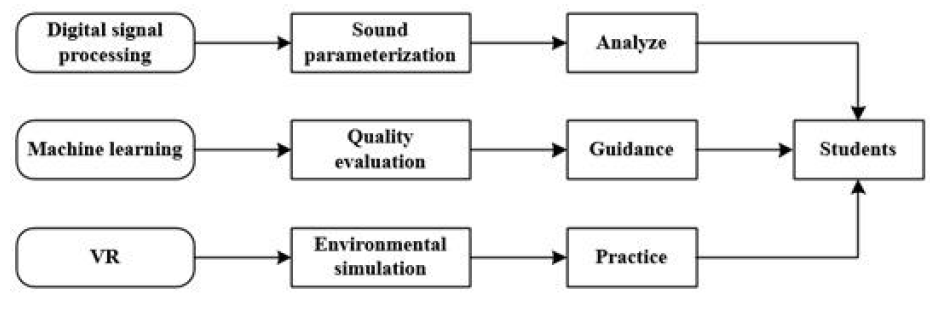
\includegraphics[width=0.7\textwidth]{images/fig2.png} 
\caption{Diagrama de integración de tecnologías clave para el análisis acústico vocal asistido: procesamiento digital de señales, machine learning y simulación de entornos. Fuente: Chen [6].}
\label{fig:fig2}
\end{figure}

Uno de los avances más significativos en este campo fue el trabajo de Martínez Ramírez, Stoller y Moffat en [2], quienes propusieron el uso de una variante de la arquitectura Wave-U-Net para la mezcla automática de batería. En ese trabajo se demostró que una red neuronal profunda puede aprender directamente la transformación de audio implicada en la mezcla sin necesidad de modelar efectos individuales por separado, y que los resultados obtenidos fueron perceptualmente indistinguibles de las mezclas realizadas por ingenieros humanos profesionales.

\begin{figure}[h!]
\centering
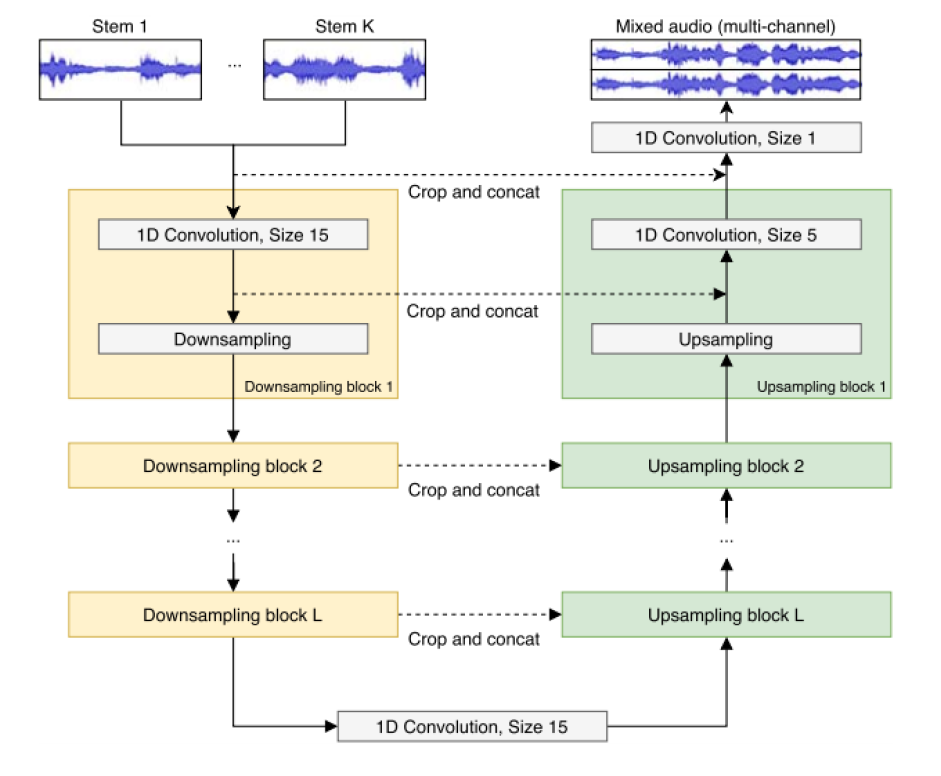
\includegraphics[width=0.9\textwidth]{images/fig3.png} 
\caption{Diagrama de bloques de la arquitectura Wave-U-Net adaptada para mezcla automática de batería, mostrando el flujo desde las pistas individuales (stems) hasta la mezcla estéreo de salida. Fuente: Martínez Ramírez et al. [2].}
\label{fig:fig3}
\end{figure}

Más recientemente, Moliner et al. en [3] introdujeron MEGAMI (\textit{Multitrack Embedding Generative Auto MIxing}), un framework generativo basado en modelos de difusión condicional que opera en un espacio de embeddings de efectos. A diferencia de los enfoques de regresión anteriores, MEGAMI modela la distribución condicional de mezclas profesionales, reconociendo que para un mismo conjunto de pistas existen múltiples mezclas igualmente válidas. Este enfoque representa un cambio de paradigma relevante: pasar de predecir una única mezcla "promedio" a generar propuestas diversas que reflejan distintas decisiones artísticas posibles.

\begin{figure}[h!]
\centering
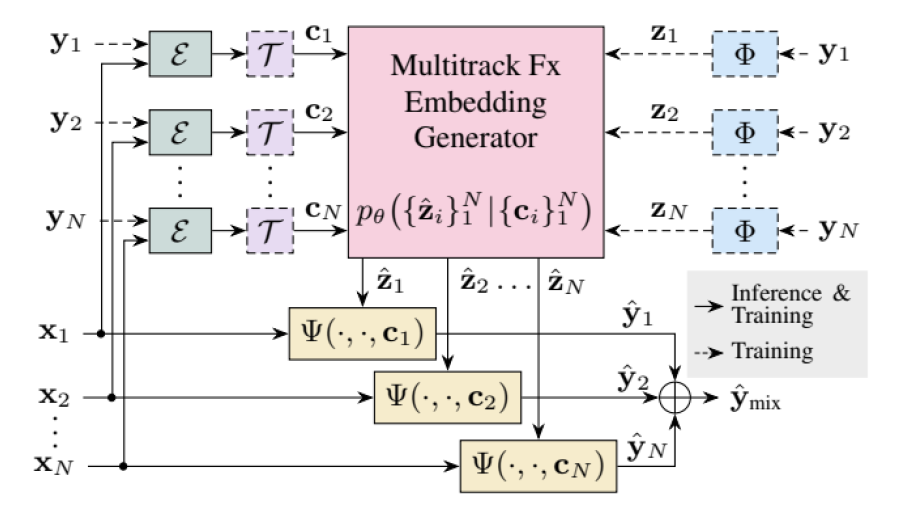
\includegraphics[width=0.9\textwidth]{images/fig4.png}
\caption{Diagrama del sistema MEGAMI, ilustrando los componentes de extracción de embeddings de efectos, el modelo de difusión condicional y el procesador de efectos por pista. Fuente: Moliner et al. [3].}
\label{fig:fig4}
\end{figure}

\subsubsection*{Sistemas inteligentes de asistencia en producción musical}

No todos los sistemas inteligentes para producción musical están orientados a la automatización completa del proceso. Existe una distinción importante y relevante, entre sistemas de mezcla completamente automáticos y herramientas de asistencia inteligente que apoyan las decisiones del usuario sin reemplazar su criterio creativo.

De Man, Reiss y Stables, en [4], identificaron esta división, clasificando las aplicaciones de mezcla automática en una escala que va desde sistemas de un sistema de caja negra sin intervención humana hasta asistentes que ofrecen un punto de partida para el ingeniero. Los autores destacan que aunque los sistemas completamente automáticos tienen aplicaciones correctas en contextos con recursos limitados como ensayos de bandas o salas pequeñas de conciertos sin ingenieros profesionales, en producción profesional la mayoría de los ingenieros prefieren herramientas que les ofrezcan control y personalización.

Esta preferencia fue confirmada empíricamente por Vanka et al. en [1], quienes investigaron la adopción de herramientas de IA en flujos de trabajo de mezcla a través de entrevistas, cuestionarios y análisis de foros de internet. Sus hallazgos identificaron tres grupos de usuarios con necesidades distintas: los amateurs, que buscan sistemas altamente autónomos que simplifiquen el proceso; los semi-profesionales, que valoran las herramientas como punto de partida y como recurso de aprendizaje; y los profesionales, que demandan control, precisión y posibilidades de personalización avanzada. Los autores señalan además que los profesionales muestran mayor aceptación hacia tecnologías asistivas y co-creativas, en las que el sistema hace sugerencias y el ingeniero tiene la decisión final.

\begin{figure}[h!]
\centering
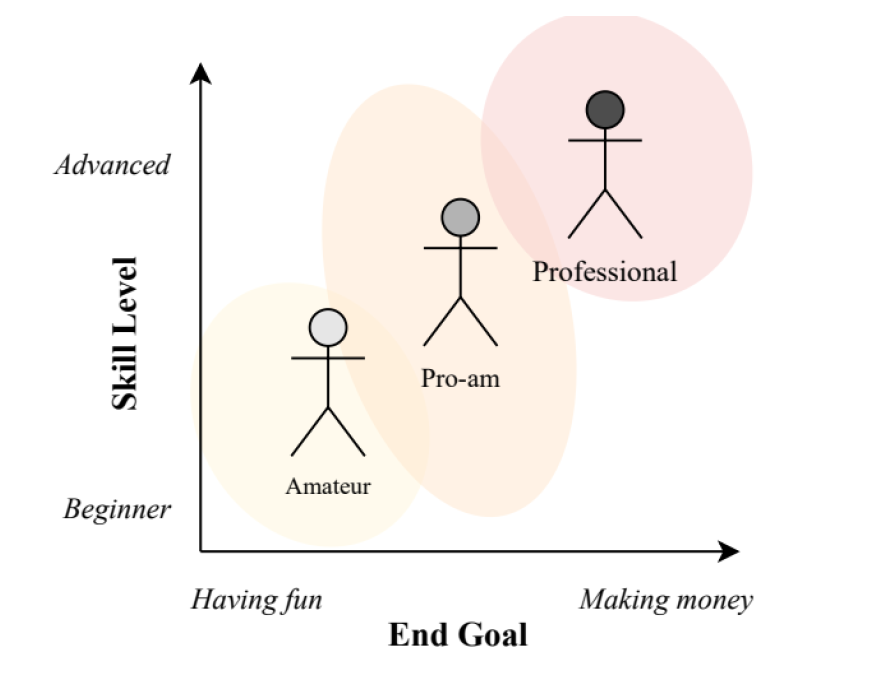
\includegraphics[width=0.7\textwidth]{images/fig5.png} 
\caption{Categorización de usuarios de herramientas inteligentes de mezcla según nivel de habilidad y objetivo final. Fuente: Vanka et al. [1].}
\label{fig:fig5}
\end{figure}

Este contexto sostiene el enfoque del presente proyecto: en lugar de buscar automatizar completamente la mezcla vocal, se propone un sistema inteligente de asistencia capaz de generar propuestas iniciales de cadenas de procesamiento que el usuario pueda ajustar según su criterio. De esta manera, el sistema actúa como un punto de partida técnicamente informado, reduciendo la incertidumbre sin limitar la libertad creativa del ingeniero de mezcla.

\subsubsection*{Sistemas inteligentes interpretables en mezcla}

Un aspecto importante dentro del desarrollo reciente de herramientas inteligentes para producción musical es la necesidad de que los sistemas no funcionen únicamente como cajas negras. En los primeros enfoques de mezcla automática, muchos modelos buscaban generar directamente una señal de audio final a partir de las pistas de entrada. Aunque este tipo de aproximación puede producir resultados técnicamente válidos, presenta una limitación importante para el usuario: no siempre permite comprender qué decisiones tomó el sistema ni modificar con precisión los procesos aplicados.

En este sentido, los sistemas interpretables buscan generar resultados que puedan ser revisados y ajustados por el ingeniero o productor dependiendo de la situación. Esto significa que en lugar de entregar únicamente una mezcla final cerrada, el sistema puede proponer parámetros de procesamiento, configuraciones de efectos o cadenas de mezcla que el usuario pueda modificar según su criterio. Steinmetz et al. [7] propone una consola de mezcla diferenciable capaz de producir parámetros legibles para el usuario, lo que permite ajustar manualmente la mezcla generada y conservar cierto grado de control creativo. Este enfoque resulta relevante para el presente proyecto, ya que la plataforma propuesta no busca reemplazar al ingeniero de mezcla, sino asistirlo en la construcción inicial de una cadena vocal ajustable.

En el caso de la mezcla vocal, la interpretabilidad adquiere una importancia particular, ya que decisiones como aplicar un filtro de paso alto, reducir resonancias, controlar sibilancias, comprimir la dinámica o añadir reverberación no responden únicamente a criterios automáticos, sino también a la intención artística de la canción. Por esta razón, una plataforma de asistencia inteligente debe permitir que el usuario comprenda la lógica general de la recomendación y pueda modificarla según las necesidades de la voz y del contexto musical.

\subsubsection*{Descriptores semánticos aplicados a la mezcla}

En la práctica de la producción musical, muchas decisiones de mezcla no se comunican únicamente mediante términos técnicos, sino también mediante descripciones sensoriales o semánticos. Es común que artistas, productores o clientes describan una voz como "opaca", "brillante", "nasal", "cálida", "agresiva", "suave" o "presente", incluso cuando no tienen conocimientos específicos sobre ecualización, compresión o procesamiento dinámico. Estos términos hacen parte del lenguaje cotidiano de la mezcla y permiten traducir una intención sonora en una posible acción técnica.

Venkatesh, Moffat y Miranda [9] exploran esta relación entre lenguaje y procesamiento de audio mediante el uso de word embeddings para traducir descriptores semánticos a configuraciones de ecualización. Su propuesta parte de la idea de que los usuarios pueden expresar objetivos sonoros en palabras y que un sistema inteligente puede aprender relaciones entre esos descriptores y ciertos comportamientos de ecualización. Este enfoque es relevante para el presente proyecto porque permite ver el asistente no solo como una herramienta que analiza datos acústicos, sino también como un sistema que puede recibir información sobre la intención sonora del usuario.

Aplicado a la mezcla vocal, esto significa que la plataforma podría relacionar descriptores como "más clara", "menos nasal" o "más cálida" con decisiones de procesamiento específicas, como aumentar la presencia en ciertas bandas de frecuencia, reducir acumulaciones en medios bajos o controlar sibilancias en la zona alta del espectro. De esta manera, el asistente podría funcionar como una conexión entre el lenguaje perceptual del usuario y las acciones técnicas propias de una cadena de mezcla vocal.

\begin{figure}[h!]
\centering
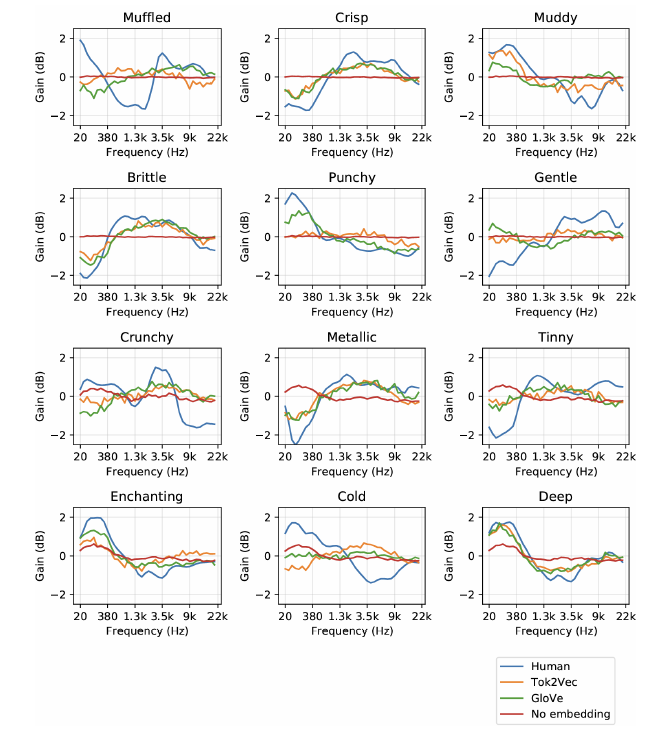
\includegraphics[width=0.9\textwidth]{images/fig6.png} 
\caption{Relación entre descriptores semánticos y configuraciones de ecualización mediante modelos de word embeddings. Fuente: Venkatesh, Moffat y Miranda [9].}
\label{fig:fig6}
\end{figure}

\subsubsection*{Contexto e intención sonora en sistemas inteligentes de mezcla}

La mezcla musical no ocurre de manera independiente. Cada decisión técnica depende del contexto de la canción, del género musical, de la intención estética, de las expectativas del artista y del nivel de experiencia del usuario. Por esta razón, una misma cadena de procesamiento vocal puede funcionar adecuadamente en un género musical y resultar inapropiada en otro. Una voz principal en pop, por ejemplo, puede requerir un tratamiento más brillante, presente y controlado, mientras que una voz en un contexto urbano, alternativo o experimental puede buscar una textura más procesada, saturada o espacial.

Lefford et al. [8] proponen que los sistemas inteligentes de mezcla deben considerar el contexto, ya que los ingenieros humanos toman decisiones no solo a partir de reglas técnicas, sino también de la situación musical, las convenciones del género y las expectativas creativas del proyecto. Desde esta perspectiva, una herramienta inteligente no debería limitarse a aplicar reglas generales de procesamiento, sino que debería adaptarse, al menos parcialmente, a las condiciones particulares de cada producción.

Este planteamiento refuerza la orientación asistiva del presente proyecto. La plataforma propuesta debe analizar la señal vocal, pero también permitir que el usuario indique información contextual básica, como el género musical, el tipo de voz, el objetivo sonoro o una referencia musical. De esta manera, la cadena sugerida no se entendería como una solución universal, sino como una propuesta inicial ajustada a una situación de mezcla específica.

\subsubsection*{Criterios objetivos de evaluación en mezcla vocal}

Aunque la mezcla musical tiene un componente subjetivo y creativo, también existen criterios técnicos que permiten evaluar ciertos aspectos de calidad sonora. Variables como el loudness, el true peak, la presencia de clipping, el rango dinámico, el balance tonal, la compresión y la compatibilidad mono pueden aportar información objetiva sobre el estado de una mezcla o de una señal procesada. Estos criterios no reemplazan la escucha crítica, pero sí permiten identificar problemas técnicos que pueden afectar la claridad, la inteligibilidad y la calidad final del audio.

Mourgela et al. [10] analiza una base de datos extensa de mezclas y masters a partir de métricas como loudness integrado, true peak, clipping, problemas de fase, compresión, amplitud estéreo y perfil tonal. Este tipo de análisis resulta útil para el presente proyecto ya que permite definir criterios técnicos que pueden integrarse en la evaluación de las cadenas vocales generadas por el sistema. En lugar de evaluar únicamente si una cadena "suena bien", se pueden observar también aspectos medibles como exceso de nivel, sobrecompresión, acumulación espectral o falta de control dinámico.

En el caso de la mezcla vocal, estos criterios pueden adaptarse al análisis de claridad, presencia, sibilancia, estabilidad dinámica y balance tonal de la voz dentro del contexto musical. Así, la validación de la plataforma puede combinar una dimensión objetiva, basada en mediciones acústicas, y una dimensión subjetiva, basada en la percepción de usuarios e ingenieros de sonido.

\subsection*{Marco referencial del proyecto}

El campo de la mezcla automática e inteligente tiene raíces que se extienden por más de una década. De Man, Reiss y Stables, en [4], ofrecen una revisión sistemática del tema que abarca desde los trabajos pioneros de Enrique Perez Gonzalez entre 2007 y 2010, quien fue el primero en proponer métodos para automatizar no solo los niveles sino también el paneo estéreo en mezcla de audio, hasta los desarrollos más recientes que incorporan machine learning. En ese recorrido se hace evidente una tendencia clara: los sistemas basados en reglas y algoritmos fueron gradualmente reemplazados por enfoques de aprendizaje automático, que demostraron mayor flexibilidad para capturar la complejidad y variabilidad del proceso de mezcla. Los autores también identifican las aplicaciones más prometedoras del campo, organizándolas en cuatro categorías: sistemas de caja negra completamente autónomos, asistentes con distintos niveles de control para el usuario, interfaces con parámetros semánticos más accesibles, y herramientas de diagnóstico y medición inteligente.

\begin{figure}[h!]
\centering
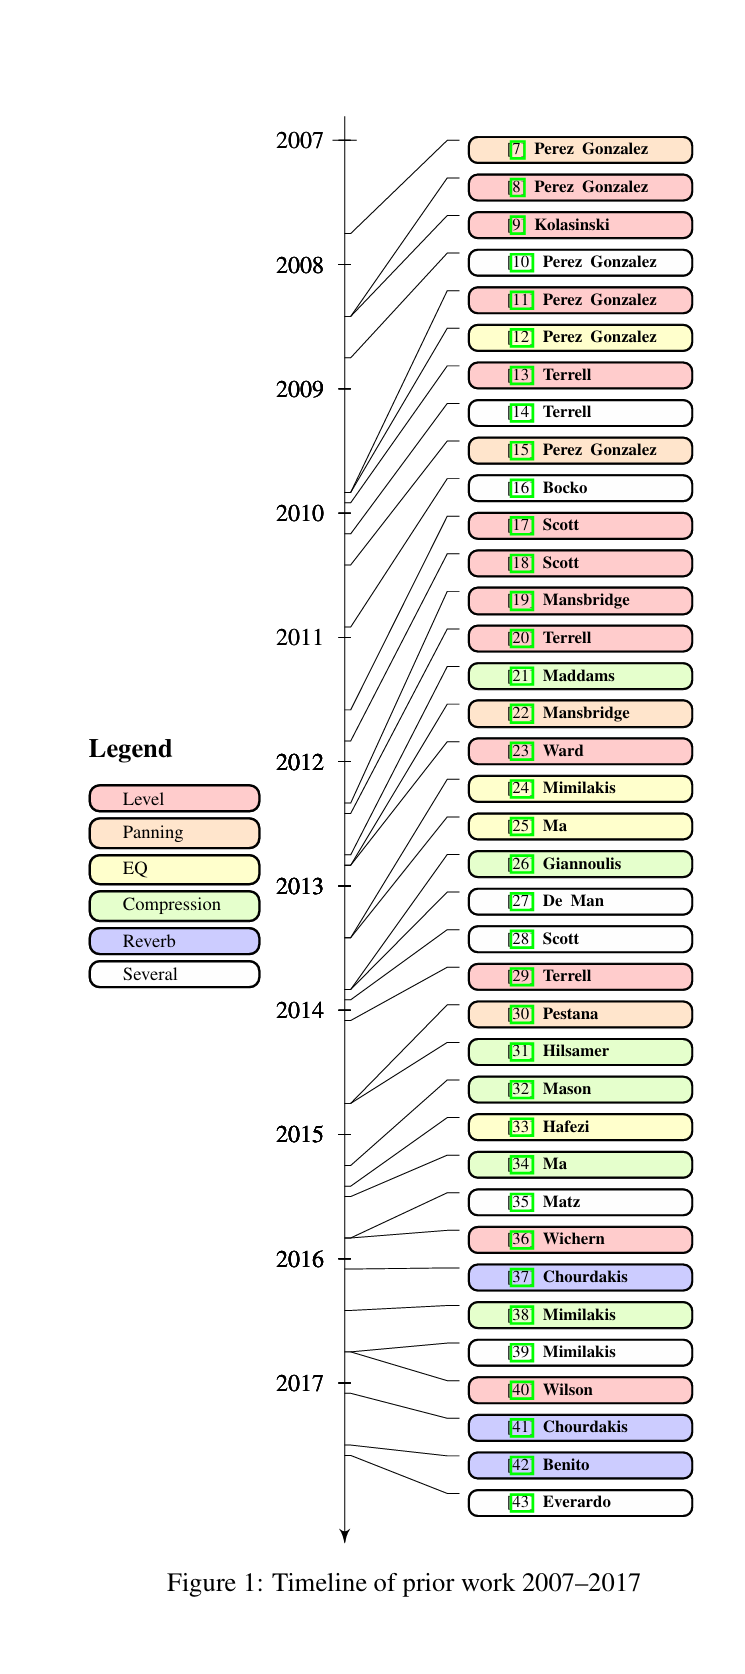
\includegraphics[width=0.7\textwidth]{images/fig7.png} 
\caption{Línea de tiempo de sistemas publicados para automatización de mezcla musical entre 2007 y 2017, clasificados por tipo de proceso automatizado. Fuente: De Man et al. [4].}
\label{fig:fig7}
\end{figure}

En el enfoque del aprendizaje profundo aplicado a la mezcla, Martínez Ramírez y Reiss, en [5], presentaron en 2017 una de las primeras propuestas formales para explorar redes neuronales profundas como herramienta de mezcla inteligente. En ese trabajo se propuso tratar el procesamiento de stems como una transformación basada en contenido, entrenando autoencoders profundos (DAE) para aprender la cadena de efectos aplicada por ingenieros profesionales a partir de grabaciones crudas. Los experimentos, llevados a cabo con grupos instrumentales de bajo, guitarra, voz y teclados mostraron que el sistema podía aprender aspectos de la transformación espectral, aunque con limitaciones notables en el caso de la voz, ya que su complejidad tímbrica y variabilidad estilística la hace significativamente más difícil de modelar. Este resultado es particularmente relevante para el presente proyecto, ya que pone de manifiesto que la mezcla vocal representa un desafío específico que justifica un sistema especializado.

Siguiendo esa línea, Martínez Ramírez, Stoller y Moffat, en [2], desarrollaron un sistema de mezcla automática de batería basado en una variante de la arquitectura Wave-U-Net, que opera directamente sobre señales de audio en el dominio temporal sin necesidad de representaciones espectrales. El sistema recibe como entrada las pistas individuales de una grabación de batería y produce como salida la mezcla estéreo completa, aprendiendo simultáneamente todas las transformaciones de audio involucradas como ganancia, paneo, ecualización y compresión dinámica sin modelarlas de manera separada. En pruebas de escucha subjetiva con veinte participantes, los resultados del modelo Wave-U-Net fueron perceptualmente indistinguibles de las mezclas realizadas por ingenieros humanos, mientras que el enfoque basado en random forests utilizado como base, obtuvo calificaciones significativamente más bajas. Este estudio resulta una evidencia sólida del potencial del aprendizaje profundo para automatizar la mezcla, pero también resalta que el éxito del modelo depende en gran medida de la consistencia y estructura del material musical utilizado.

Una respuesta a esa limitación fue explorada por Vanka et al. en [1], quienes investigaron de manera sistemática la adopción de herramientas de IA en flujos de trabajo de mezcla musical, prestando especial atención a las expectativas y actitudes de distintos grupos de usuarios. A través de entrevistas con ingenieros profesionales, cuestionarios con semi-profesionales y análisis de foros de internet, los autores confirmaron que las necesidades de los usuarios varían según su nivel de experiencia. Los amateurs buscan soluciones automatizadas que les permitan tratar su música sin necesidad de dominar los aspectos técnicos del proceso de mezcla; los semi-amateurs utilizan las herramientas como punto de partida y como recurso de aprendizaje y los profesionales, que ya cuentan con flujos de trabajo establecidos, prefieren herramientas que asistan y co-creativas que les ofrezcan control y opciones de personalización avanzada. Una observación importante del estudio es que el 54\% de ingenieros entrevistados no utiliza herramientas de IA en sus flujos de trabajo, lo que sugiere que la adopción todavía enfrenta problemas relacionados con la calidad de los resultados, la integración en flujos de trabajo existentes y la confianza en los sistemas automatizados.

Moliner et al. en [3] introdujeron en 2025 MEGAMI, el primer framework generativo para mezcla automática de música multipista. A diferencia de todos los enfoques anteriores que trataban la mezcla como un problema de regresión determinística (prediciendo una única mezcla a partir de un conjunto de pistas), MEGAMI modela la distribución condicional de mezclas profesionales, reconociendo explícitamente que múltiples mezclas válidas pueden existir para las mismas entradas. El sistema opera en un espacio de embeddings de efectos, separando las decisiones de mezcla del contenido musical mediante representaciones aprendidas. En la evaluación objetiva, MEGAMI superó consistentemente a todos los sistemas de línea de base, y en las pruebas de escucha subjetiva se acercó a la calidad de las mezclas realizadas por ingenieros humanos, incluso superándolos en algunos géneros. Esta investigación es de las más recientes en cuanto sistemas automatizados de mezcla, estableciendo un referente técnico importante para el presente proyecto, que busca desarrollar un sistema especializado en la voz con un enfoque asistivo en lugar de completamente automático.

A partir de este mismo problema por evitar sistemas cerrados o poco interpretables, Steinmetz et al. [7] propusieron un enfoque de mezcla multipista basado en una consola de mezcla diferenciable compuesta por efectos neuronales de audio. A diferencia de los modelos que generan directamente una señal final, este sistema estima parámetros de mezcla legibles por el usuario lo que permite revisar y ajustar manualmente el resultado generado. El trabajo resulta importante para el presente proyecto porque plantea una alternativa intermedia entre la automatización completa y la asistencia controlada: el sistema puede aprender convenciones de mezcla a partir de datos reales pero conserva una estructura cercana al flujo de trabajo tradicional del ingeniero basada en parámetros, canales y procesos ajustables. Esta lógica se relaciona directamente con la plataforma propuesta, ya que el objetivo no es entregar una mezcla vocal cerrada sino sugerir una cadena de procesamiento que pueda ser modificada por el usuario.

Desde una perspectiva más conceptual, Lefford et al. [8] introdujeron la noción de sistemas inteligentes de mezcla conscientes del contexto. Los autores señalan que las decisiones de mezcla no dependen únicamente de reglas técnicas, sino también del género musical, la intención emocional, las expectativas del cliente, el entorno de trabajo y la experiencia del ingeniero. Esta investigación permite ampliar la comprensión del problema ya que muestra que una herramienta inteligente no debería limitarse a analizar la señal de audio de manera aislada, sino que también debería considerar las condiciones particulares de uso. Para el presente proyecto este planteamiento es importante porque justifica que la plataforma incorpore información contextual como el género, el tipo de voz, la intención sonora o una referencia musical.

En relación con la comunicación entre usuario y sistema, Venkatesh, Moffat y Miranda [9] estudiaron el uso de word embeddings para la ecualización automática en mezcla de audio. Su investigación propone traducir descriptores semánticos a configuraciones de ecualización, permitiendo que términos como "calida", "brillante", "oscura" o "suave" puedan relacionarse con curvas de EQ. Este antecedente resulta especialmente útil para el desarrollo de una plataforma de asistencia en mezcla vocal, ya que muchos productores y artistas no comunican sus objetivos sonoros mediante parámetros técnicos, sino mediante descripciones perceptuales. Por lo tanto, la incorporación de descriptores semánticos podría facilitar que el usuario exprese la intención de la voz de una manera más intuitiva, mientras el sistema traduce esa intención en una posible recomendación de procesamiento.

Por otra parte, Mourgela et al. [10] aportan una perspectiva basada en el análisis de grandes volúmenes de datos reales de mezclas y masters. Su estudio examina más de 218.000 entradas provenientes de una plataforma web de análisis de audio, considerando variables como loudness integrado, true peak, clipping, compresión, problemas de fase, compatibilidad mono, amplitud estéreo y perfil tonal. Esto es realmente importante para el presente proyecto porque permite justificar la selección de métricas objetivas para evaluar las cadenas generadas por el sistema. Aunque la mezcla vocal mantiene un componente subjetivo, el uso de criterios técnicos medibles permite verificar si las propuestas cumplen condiciones básicas de calidad sonora, como evitar distorsión, controlar la dinámica y mantener un balance tonal coherente.

Finalmente, Vanka et al. [11] desarrollaron Diff-MST, un sistema de transferencia de estilo de mezcla basado en una consola diferenciable, un controlador tipo transformer y una función de pérdida orientada al estilo de producción. El sistema recibe pistas crudas y una canción de referencia para estimar parámetros de efectos dentro de una consola de mezcla, permitiendo generar una mezcla con características similares a la referencia y manteniendo la posibilidad de ajustes posteriores. Este antecedente resulta importante porque introduce la referencia musical como una fuente de información para orientar las decisiones del sistema. En el contexto del presente proyecto, esta idea permite pensar la cadena de mezcla vocal no solo desde las características acústicas de la voz, sino también desde el estilo sonoro que el usuario desea alcanzar.


